\chapter{Data}

InfectX is an \gls{rtd} project funded by SystemsX, the Swiss initiative for systems biology with the goal of studying and identifying components of the human infectome for a set of bacterial and viral pathogens. A central effort consists of generating kinome- and genome-wide \gls{sirna} screens for each of the investigated pathogens, capturing image data and performing image analysis. The acquired data is publicly available on the internet at \href{http://www.infectx.ch/databrowser}{the InfectX website}.

\section{InfectX Workflow}
Due to the large scale accompanied by screening multiple libraries, using numerous pathogens and desiring replicates, several labs were involved in carrying out wet-lab experimentation. In order to obtain reproducible results, a strong emphasis was put on developing unified procedures for cell culture, \gls{sirna} transfection, pathogen infection and imaging. Figure \ref{fig:infectx} summarizes the central steps, beginning with \gls{sirna} libraries arrayed onto 384-well plates that are used for transfection of added cells, carrying on with pathogen infection, subsequent microscopic imaging and concluding with computational image analysis. Much of the information contained in this chapter has been published by \cite{Ramo2014} and is summarized for the reader's convenience.

\begin{figure}
  \centering
  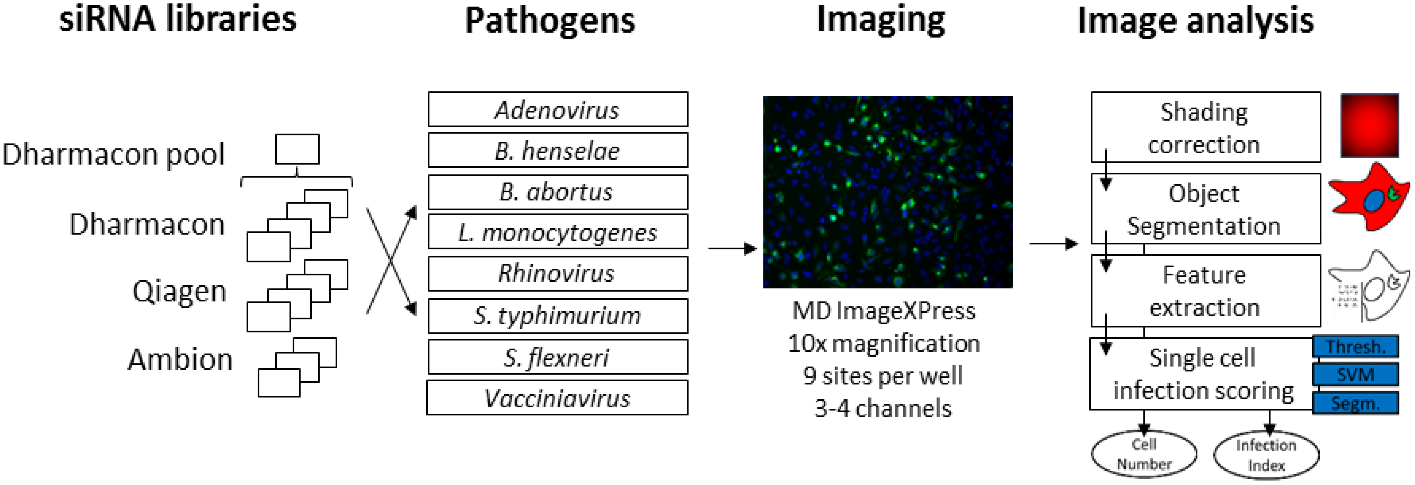
\includegraphics[width=0.95\textwidth]{infectx}
  \caption[InfectX RNAi data acquisition and analysis workflow.]{A total of 11 single \gls{sirna} libraries, pdroduced by 3 separate manufacturers, (4 from Dharmacon, 4 from Quiagen and 3 from Ambion), as well as one pooled library (Dharmacon) were screened with 8 pathogens. Plates were imaged under wide-field microscopes and the resulting images run through an image analysis pipeline. \citep{Ramo2014}.}
  \label{fig:infectx}
\end{figure}

The model system chosen for investigation is HeLa (ATCC CCL-2), the oldest and most wide spread human cell line and a proven system for studying infelicitous disease\footnote{Collected 60 years ago from a cervical adenocarcinoma, these epithelial cells have led to much insight into human cell biology. Prior to their discovery, attempts at growing human tissue in vitro were futile and development of protocols for sustaining cancerous human tissue was thought to hold great promise for cancer research. One of the early successes involving HeLa cells was the development a polio vaccine. For this endeavor, a large amount of human cells were needed and the installment of a production facility capable of meeting the high demand might have contributed significantly to the predominance of these cells. \citep{Masters2002}}. Culturing was performed at \SI{37}{\celsius}, under 5\% \ce{CO2} atmosphere for maintaining optimal pH, using \gls{dmem}  supplemented with 10\% inactivated \gls{fbs}, both supplied by Invitrogen.

While genome-wide \gls{sirna} screens were also produced within the InfectX framework, this report focuses on kinome-wide investigations. Introduced by \cite{Manning2002}, the term kinome refers to the subset of genes encoding protein kinases\footnote{Kinases are part of the larger enzymatic family of transferases and catalyze phosphorylation reactions of the form
\begin{equation}
  \ce{A\bond{-}O\bond{-}PO3^{-2} + H\bond{-}X\bond{-}B <=>> B\bond{-}X\bond{-}O\bond{-}PO3^{-2} + H\bond{-}O\bond{-}A} \label{eq:kinase}
\end{equation}
where A represents the donating (typically \gls{atp}) and B the accepting molecule. Kinases are further subdivided according to the type of acceptor which can be an alcohol, carboxy, nitrogenous or phosphate group, or in case of protein kinases, a tyrosine, serine, threonine or histidine residue.
\begin{align}
  \cee{A\bond{-}O\bond{-}B + H\bond{-}O\bond{-}PO3^{-2} &<=>> A\bond{-}O\bond{-}PO3^{-2} + H\bond{-}O\bond{-}B} \label{eq:phosphorylase} \\
  \cee{A\bond{-}O\bond{-}PO3^{-2} + H\bond{-}OH &<=>> A\bond{-}OH + H\bond{-}O\bond{-}PO3^{-2}} \label{eq:phosphatases}
\end{align}
Phosphorylases are a further group of transferases that involve phosphate but unlike kinases, they utilize inorganic phosphate sources (\ref{eq:phosphorylase}). Often phosphorylases are involved in breaking down biological polymers such as polysaccharides and polynucleotides. Finally, phosphatases catalyze the reverse reaction, the removal of a phosphate group (\ref{eq:phosphatases}).}. As phosphorylation reactions have been identified to constitute the most widespread signaling mechanism in eukaryotic cells, the set of 518 genes identified by \citeauthor{Manning2002} are a popular target for functional genomics studies. Up to 30\% of intracellular proteins may be phosphorylated, leading to 20000 phosphoprotein states, all regulated by expression of varyingly substrate specific kinases \citep{Johnson2005}. Due to the importance of kinases for cell behavior, they represent a major drug target in cancer therapeutics and might therefore also be attractive for \gls{hdt}.

In order to offset potential bias introduced by \gls{sirna} design paradigms employed by manufacturers, libraries from three different companies (Abion, Dharmacon and Qiagen) were obtained. To further account for the effect of \glspl{ote}, several \gls{sirna} sequences per target were used for both pooled and unpooled experiments. The Ambion Silencer Select Human Kinase siRNA Library V4 targets 710 genes of kinases and kinome-associated proteins with 3 sequences each, while the Qiagen HP OnGuard Human Kinase siRNA Set V4.1 comprises of 718 targets and 4 \glspl{sirna} per gene. The Dharmacon Human ON-TARGETplus siRNA Protein Kinase Libraries are designed with 715 genes in mind and are both available in 1 \gls{sirna} per well (unpooled) and 4 \glspl{sirna} per well (pooled) formats.

\begin{table}
  \centering
  \caption[Number of replicates performed for each of the pathogens and \gls{sirna} libraries.]{Number of replicates performed for each of the pathogens and \gls{sirna} libraries. The primary values indicate how many were performed in total while the value in parenthesis represents the number of screens that turned out to be unusable and had to be discarded. The effectively available number of replicates is the difference between the two. \citep{Ramo2014}}
  \label{tab:infectx-replicates}
  \footnotesize
  \begin{tabular}{L{0.2\linewidth}C{0.13\linewidth}C{0.13\linewidth}C{0.13\linewidth}C{0.15\linewidth}}
    Pathogen &
      Dharmacon (1x pooled) &
      Ambion (3x single) &
      Quiagen (4x single) &
      Dharmacon (4x single) \\
    \hline 
    \textit{B. abortus} &
      8 (1 rem.) &
      2 &
      1 &
      2 \\
    \textit{B. henselae} &
      5 (1 rem.) &
      4 (1 rem.) &
      2 (1 rem.) &
      1 \\
    \textit{L. monocytogenes} &
      4 &
      4 (2 rem.) &
      1 &
      1 \\
    \textit{S. flexneri} &
      6 (2 rem.) &
      2 &
      1 &
      1 \\
    \textit{S.} typhimurium &
      7 (4 rem.) &
      3 &
      1 &
      1 \\
    adenovirus &
      8 (1 rem.) &
      2 &
      1 &
      1 \\
    rhinovirus &
      8 (2 rem.) &
      2 &
      1 &
      1 \\
    vaccinia virus &
      2 (1 rem.) &
      2 &
      1 &
      1 \\
    \hline
  \end{tabular}
\end{table}

Depending on library and pathogen, screens were repeated 1--8 times (see table \ref{tab:infectx-replicates}). The primary values denote the total number of replicated performed and the values in parenthesis indicate the number of screens that had to be removed due to issues with transfection, weak signal intensities or usage of a protocol other than the one eventually agreed upon. The Dharmacon pooled screen was used for optimizing the assay procedures which is why for almost all pathogens some replicates had to be removed. The number of available screens is the difference between primary and parenthesized values.

\section{RNA Interference Protocols}
Central to the \gls{sirna} screens produced by InfectX was the effort to develop unified protocols for wet-tab experiments and subsequent analysis. While this approach was successfully implemented for many aspects, some deviations among the pathogens are inevitable, while others are intentionally developed to achieve similar phenotypes. Table \ref{tab:infectx-differences} summarizes some key parameters that vary between pathogens, which include seeded cell number, \gls{moi} and infection times, all optimized to yield infection rates that are of comparable magnitude. The target value for cell number was 1500 per well in order to create densely populated areas interspersed with some empty spaces, leading to cells living on colony edges and infection rates of 30--50\% were aimed for. Pathogen properties made it in some cases impossible th hit these goals and infection rate for \textit{B. abortus} remained low (\tilde 5\%), while being high in \textit{B. henselae} (\tilde 90\%) despite best efforts.

\setlength{\tabcolsep}{0.1em}
\begin{table}
  \begin{minipage}{\textwidth}
  \centering
  \caption[Differences in assay protocols among the 8 pathogens.]{Despite putting much emphasis on using identical protocols throughout all screens, some assay parameters were fine-tuned in order to obtain phenotypes such as infection and cell counts that are similar among the investigated pathogens. \citep{Ramo2014}}
  \label{tab:infectx-differences}
  \footnotesize
  \begin{tabular}{L{0.17\linewidth}C{0.09\linewidth}C{0.09\linewidth}C{0.09\linewidth}C{0.09\linewidth}C{0.09\linewidth}C{0.09\linewidth}C{0.10\linewidth}C{0.10\linewidth}}
    Pathogen &
      \mcrot{1}{l}{60}{Seeded cell number} &
      \mcrot{1}{l}{60}{\Acrshort{moi}} &
      \mcrot{1}{l}{60}{Pathogen entry time} &
      \mcrot{1}{l}{60}{Total infection time} &
      \mcrot{1}{l}{60}{DNA stain} &
      \mcrot{1}{l}{60}{Actin stain\footnote{Phalloidin-based actin stains were supplied by Dyomics and depending on absorption wavelength, different imaging channels were used: GFP for DY-495, RFP for DY-547 and Cy5 for DY-647.}} &
      \mcrot{1}{l}{60}{Pathogen stain} &
      \mcrot{1}{l}{60}{Additional stain\footnote{The Cy3 channel was used Alexa546, while Cy5 was used for Alexa647 during imaging.}} \\
    \hline 
    \textit{B. abortus} &
      500 &
      10000 &
      \SI{4}{\hour} &
      \SI{44}{\hour} &
      DAPI &
      DY-547 &
      GFP &
      - \\
    \textit{B. henselae} &
      300 &
      400 &
      \SI{24}{\hour} &
      \SI{24}{\hour} &
      DAPI &
      DY-547 &
      GFP &
      - \\
    \textit{L. monocytogenes} &
      600 &
      25 &
      \SI{1}{\hour} &
      \SI{5}{\hour} &
      DAPI &
      DY-647 &
      GFP &
      Alexa546 \\
    \textit{S. flexneri} &
      600 &
      15 &
      \SI{30}{\minute} &
      \SI{3.5}{\hour} &
      Hoechst &
      DY-495 &
      DsRed &
      Alexa647 \\
    \textit{S.} typhimurium &
      550 &
      80 &
      \SI{20}{\minute} &
      \SI{4}{\hour} &
      DAPI &
      DY-547 &
      GFP &
      - \\
    adenovirus &
      700 &
      0.1 &
      \SI{16}{\hour} &
      \SI{16}{\hour} &
      DAPI &
      DY-647 &
      GFP &
      - \\
    rhinovirus &
      1000 &
      8 &
      \SI{7}{\hour} &
      \SI{7}{\hour} &
      DAPI &
      DY-647 &
      GFP &
      - \\
    vaccinia virus &
      600 &
      0.125 &
      \SI{1}{\hour}\slash \SI{8}{\hour}\footnote{The two values stand for primary and secondary infection times, respectively. The same goes for pathogen dyes.} &
      \SI{24}{\hour} &
      Hoechst &
      DY-647 &
      GFP\slash RFP &
      - \\
  \end{tabular}
  \end{minipage}
\end{table}

The usage of control wells enables diagnosis of possible problems that may occur in RNAi screens, including cytotoxicity of \gls{sirna}, low transfection yields, failure of RNAi pathway induction, dominance of non-specific responses, and therefore should be embedded in every assay plate. Three types of control experiments are typically employed: positive, negative and mock (no \gls{sirna} treatment). Positive controls are used to confirm expected response, while negative controls help distinguish sequence specific from unspecific effects, and mock experiments help to establish a baseline \citep{Sittampalam2004}.

Positive controls ideally constitute of \glspl{sirna} with known effect on the assay under investigation and are therefore often unavailable beforehand. Instead, controls to check transfection efficiency and reporter quality are usually employed. One straightforward possibility for monitoring delivery is by targeting a gene that is vital to the cell. \Gls{kif11}, for example is a gene involved in cell cycle progression, the down-regulation of which is induces apoptosis. Furthermore there are mixtures of \glspl{sirna} available (e.g. AllStars Hs Cell Death Control siRNA by Qiagen) optimized for killing cells by targeting several ubiquitously expressed genes essential for cell survival. The downside of assessing transfection by killing cells is that a potentially toxic effect of the delivery mechanism itself may be masked. This can be mitigated by either performing negative control experiments (which should be done anyways) or by targeting housekeeping genes that are abundantly expressed but do not affect cell viability. Dharmacon suggests three such genes, \gls{ppib}, \gls{gapdh} and \gls{lmna}, for which they sell specially branded control \glspl{sirna} (as does Ambion).

Fluorescent dyes are also frequently employed in positive control experiments, typically by labeling \gls{sirna}, allowing for visual inspection of reagent localization within the cell (nuclear uptake indicates efficient transfection), or by targeting reporter genes. The latter method either allows for confirming that the reporting mechanism (usually expression of \gls{gfp} or luciferase) works as intended, or establishing that \gls{sirna} transfection was successful. Again, \gls{sirna} products targeting the commonly used reporter genes are readily available from manufacturers.

\renewcommand{\arraystretch}{1.1}
\setlength{\tabcolsep}{0.14em}
\begin{table}
\begin{minipage}{\textwidth}
  \centering
  \caption[Control experiments used in the different screens.]{Depending on screen type and pathogen, different genes were targeted for control experiments. Abbreviations: AU, Ambion unpooled; DP, Dharmacon pooled; DU, Dharmacon unpooled; and QU, Qiagen unpooled.}
  \label{tab:infectx-control}
  \footnotesize
  % latex table generated in R 3.2.0 by xtable 1.7-4 package
% Fri Aug  7 21:19:25 2015
\begin{tabular}{rllllllllllllllllllllllllllllllll}
  & \begin{sideways} Adeno AU \end{sideways} & \begin{sideways} Adeno DP \end{sideways} & \begin{sideways} Adeno DU \end{sideways} & \begin{sideways} Adeno QU \end{sideways} & \begin{sideways} \textit{Bartonella} AU \end{sideways} & \begin{sideways} \textit{Bartonella} DP \end{sideways} & \begin{sideways} \textit{Bartonella} DU \end{sideways} & \begin{sideways} \textit{Bartonella} QU \end{sideways} & \begin{sideways} \textit{Brucella} AU \end{sideways} & \begin{sideways} \textit{Brucella} DP \end{sideways} & \begin{sideways} \textit{Brucella} DU \end{sideways} & \begin{sideways} \textit{Brucella} QU \end{sideways} & \begin{sideways} \textit{Listeria} AU \end{sideways} & \begin{sideways} \textit{Listeria} DP \end{sideways} & \begin{sideways} \textit{Listeria} DU \end{sideways} & \begin{sideways} \textit{Listeria} QU \end{sideways} & \begin{sideways} Rhino AU \end{sideways} & \begin{sideways} Rhino DP \end{sideways} & \begin{sideways} Rhino DU \end{sideways} & \begin{sideways} Rhino QU \end{sideways} & \begin{sideways} \textit{Salmonella} AU \end{sideways} & \begin{sideways} \textit{Salmonella} DP \end{sideways} & \begin{sideways} \textit{Salmonella} DU \end{sideways} & \begin{sideways} \textit{Salmonella} QU \end{sideways} & \begin{sideways} \textit{Shigella} AU \end{sideways} & \begin{sideways} \textit{Shigella} DP \end{sideways} & \begin{sideways} \textit{Shigella} DU \end{sideways} & \begin{sideways} \textit{Shigella} QU \end{sideways} & \begin{sideways} Vaccinia AU \end{sideways} & \begin{sideways} Vaccinia DP \end{sideways} & \begin{sideways} Vaccinia DU \end{sideways} & \begin{sideways} Vaccinia QU \end{sideways} \\ 
  \hline
ARF1 &  &  &  &  &  &  &  &  &  &  &  &  &  &  &  &  &  &  &  &  &  &  &  &  &  &  & \checkmark &  &  &  &  &  \\ 
  ARPC3 & \checkmark & \checkmark & \checkmark & \checkmark & \checkmark & \checkmark & \checkmark & \checkmark & \checkmark & \checkmark & \checkmark & \checkmark & \checkmark & \checkmark & \checkmark & \checkmark & \checkmark & \checkmark & \checkmark & \checkmark & \checkmark & \checkmark & \checkmark & \checkmark & \checkmark & \checkmark & \checkmark & \checkmark & \checkmark & \checkmark & \checkmark & \checkmark \\ 
  ATP6V1A & \checkmark & \checkmark & \checkmark & \checkmark & \checkmark & \checkmark & \checkmark & \checkmark & \checkmark & \checkmark & \checkmark & \checkmark & \checkmark & \checkmark & \checkmark & \checkmark & \checkmark & \checkmark & \checkmark & \checkmark & \checkmark & \checkmark & \checkmark & \checkmark & \checkmark & \checkmark & \checkmark & \checkmark & \checkmark & \checkmark & \checkmark & \checkmark \\ 
  Abi1 &  &  &  & \checkmark &  &  &  & \checkmark &  &  &  & \checkmark &  &  &  & \checkmark &  &  &  & \checkmark &  &  &  & \checkmark &  &  &  & \checkmark &  &  &  & \checkmark \\ 
  CBL &  &  &  &  &  &  &  &  &  &  &  &  &  & \checkmark & \checkmark &  &  &  &  &  &  &  &  &  &  &  &  &  &  &  &  &  \\ 
  CDC42 & \checkmark & \checkmark & \checkmark & \checkmark & \checkmark & \checkmark & \checkmark &  & \checkmark & \checkmark & \checkmark &  & \checkmark & \checkmark & \checkmark &  & \checkmark & \checkmark & \checkmark & \checkmark & \checkmark & \checkmark & \checkmark &  & \checkmark & \checkmark & \checkmark &  & \checkmark & \checkmark & \checkmark & \checkmark \\ 
  CDH4 &  &  &  & \checkmark &  &  &  & \checkmark &  &  &  & \checkmark &  &  &  & \checkmark &  &  &  & \checkmark &  &  &  & \checkmark &  &  &  & \checkmark &  &  &  & \checkmark \\ 
  CFL1 &  &  &  &  &  &  &  &  &  &  &  &  &  &  &  &  &  &  &  &  &  &  & \checkmark &  &  &  &  &  &  &  &  &  \\ 
  CHUK &  &  &  &  &  &  &  &  &  &  &  &  &  &  &  &  &  &  &  &  &  &  &  &  &  &  & \checkmark &  &  &  &  &  \\ 
  CLTC &  &  &  &  &  &  &  &  &  &  &  &  &  & \checkmark & \checkmark &  &  &  &  &  &  &  &  &  &  &  &  &  &  &  &  &  \\ 
  DNM2 &  &  &  &  &  &  &  &  &  &  &  &  &  & \checkmark & \checkmark &  &  &  &  &  &  &  &  &  &  &  &  &  &  &  &  &  \\ 
  FRAP1 &  &  & \checkmark & \checkmark &  &  &  & \checkmark &  &  &  & \checkmark &  &  &  & \checkmark &  &  & \checkmark & \checkmark &  &  &  & \checkmark &  &  &  & \checkmark &  &  &  & \checkmark \\ 
  GFP 1\footnote{\label{fn:gfp}GFP targeting \gls{sirna} sequences are provided by Ambion (Ambion Silencer eGFP; GFP 1) and Dharmacon (GFP Duplex III; GFP 2).} & \checkmark &  &  &  & \checkmark &  &  &  & \checkmark &  &  &  & \checkmark &  &  &  & \checkmark &  &  &  & \checkmark &  &  &  & \checkmark &  &  &  & \checkmark &  &  &  \\ 
  GFP 2\textsuperscript{\ref{fn:gfp}} & \checkmark & \checkmark & \checkmark & \checkmark &  & \checkmark & \checkmark & \checkmark &  & \checkmark & \checkmark & \checkmark &  & \checkmark & \checkmark & \checkmark & \checkmark & \checkmark & \checkmark & \checkmark &  & \checkmark & \checkmark & \checkmark &  & \checkmark & \checkmark & \checkmark &  & \checkmark & \checkmark & \checkmark \\ 
  ITGAV &  &  &  &  &  &  &  &  &  &  &  &  &  &  &  &  &  &  &  &  &  &  & \checkmark &  &  &  &  &  &  &  &  &  \\ 
  ITGB1 &  &  &  & \checkmark &  &  & \checkmark & \checkmark &  &  & \checkmark & \checkmark &  &  &  & \checkmark &  &  &  & \checkmark &  &  &  & \checkmark &  &  &  & \checkmark &  &  &  & \checkmark \\ 
  Kif11 & \checkmark & \checkmark & \checkmark & \checkmark & \checkmark & \checkmark & \checkmark & \checkmark & \checkmark & \checkmark & \checkmark & \checkmark & \checkmark & \checkmark & \checkmark & \checkmark & \checkmark & \checkmark & \checkmark & \checkmark & \checkmark & \checkmark & \checkmark & \checkmark & \checkmark & \checkmark & \checkmark & \checkmark & \checkmark & \checkmark & \checkmark & \checkmark \\ 
  Kill\footnote{A positive control cell killer is provided by Qiagen (AllStars Hs Cell Death Control)} &  &  &  & \checkmark &  &  &  & \checkmark &  &  &  & \checkmark &  &  &  & \checkmark &  &  &  & \checkmark &  &  &  & \checkmark &  &  &  & \checkmark &  &  &  & \checkmark \\ 
  MAP3K7 &  &  &  & \checkmark &  &  &  & \checkmark &  &  &  & \checkmark &  &  &  & \checkmark &  &  &  & \checkmark &  &  &  & \checkmark &  &  & \checkmark & \checkmark &  &  &  & \checkmark \\ 
  MET &  &  &  & \checkmark &  &  &  & \checkmark &  &  &  & \checkmark &  & \checkmark & \checkmark & \checkmark &  &  &  & \checkmark &  &  &  & \checkmark &  &  &  & \checkmark &  &  &  & \checkmark \\ 
  MOCK & \checkmark & \checkmark & \checkmark & \checkmark & \checkmark & \checkmark & \checkmark & \checkmark & \checkmark & \checkmark & \checkmark & \checkmark & \checkmark & \checkmark & \checkmark & \checkmark & \checkmark & \checkmark & \checkmark & \checkmark & \checkmark & \checkmark & \checkmark & \checkmark & \checkmark & \checkmark & \checkmark & \checkmark & \checkmark & \checkmark & \checkmark & \checkmark \\ 
  NOD1 &  &  &  &  &  &  &  &  &  &  &  &  &  &  &  &  &  &  &  &  &  &  &  &  &  &  & \checkmark &  &  &  &  &  \\ 
  PAK1 &  &  &  &  &  &  &  &  &  &  &  &  &  &  &  &  &  &  &  &  &  &  &  &  &  &  &  &  &  &  & \checkmark & \checkmark \\ 
  PI4KA &  &  &  &  &  &  &  &  &  &  &  &  &  &  &  &  &  &  &  &  &  &  &  &  &  &  & \checkmark &  &  &  &  &  \\ 
  PI4KB &  &  &  & \checkmark &  &  &  & \checkmark &  &  &  & \checkmark &  &  &  & \checkmark &  &  &  & \checkmark &  &  &  & \checkmark &  &  &  & \checkmark &  &  &  & \checkmark \\ 
  PIK3R1 &  &  &  &  &  &  &  &  &  &  &  &  &  & \checkmark & \checkmark &  &  &  &  &  &  &  &  &  &  &  &  &  &  &  &  &  \\ 
  PRKCA &  &  & \checkmark & \checkmark &  &  &  &  &  &  &  &  &  &  &  &  &  &  & \checkmark & \checkmark &  &  &  &  &  &  &  &  &  &  &  &  \\ 
  PSMA6 &  &  &  &  &  &  &  &  &  &  &  &  &  &  &  &  &  &  &  &  &  &  &  &  &  &  &  &  &  &  & \checkmark & \checkmark \\ 
  PSMC3 &  &  &  & \checkmark &  &  &  & \checkmark &  &  &  & \checkmark &  &  &  & \checkmark &  &  &  & \checkmark &  &  &  & \checkmark &  &  &  & \checkmark &  &  & \checkmark & \checkmark \\ 
  PXN &  &  & \checkmark & \checkmark &  &  & \checkmark & \checkmark &  &  & \checkmark & \checkmark &  &  &  & \checkmark &  &  & \checkmark & \checkmark &  &  &  & \checkmark &  &  &  & \checkmark &  &  &  & \checkmark \\ 
  RAB7A &  &  &  &  &  &  &  &  &  &  &  &  &  &  &  &  &  &  &  &  &  &  & \checkmark &  &  &  &  &  &  &  &  &  \\ 
  RAC1 &  &  & \checkmark & \checkmark &  &  & \checkmark &  &  &  & \checkmark &  &  &  &  &  &  &  & \checkmark & \checkmark &  &  &  &  &  &  &  &  &  &  & \checkmark & \checkmark \\ 
  Rab2 &  &  &  &  &  &  & \checkmark &  &  &  & \checkmark &  &  &  &  &  &  &  &  &  &  &  &  &  &  &  &  &  &  &  &  &  \\ 
  SNX9 &  &  & \checkmark & \checkmark &  &  &  &  &  &  &  &  &  &  &  &  &  &  & \checkmark & \checkmark &  &  &  &  &  &  &  &  &  &  &  &  \\ 
  Scra 1\footnote{\label{fn:scram}Scrambled \gls{sirna} sequences are provided by Ambion (Silencer Select Negative Control; Scra 1) and Dharmacon (ON-TARGETplus Non-targeting Control; Scra 2).} & \checkmark &  &  &  & \checkmark &  &  &  & \checkmark &  &  &  & \checkmark &  &  &  & \checkmark &  &  &  & \checkmark &  &  &  & \checkmark &  &  &  & \checkmark &  &  &  \\ 
  Scra 2\textsuperscript{\ref{fn:scram}} & \checkmark & \checkmark & \checkmark & \checkmark &  & \checkmark & \checkmark & \checkmark &  & \checkmark & \checkmark & \checkmark &  & \checkmark & \checkmark & \checkmark & \checkmark & \checkmark & \checkmark & \checkmark &  & \checkmark & \checkmark & \checkmark &  & \checkmark & \checkmark & \checkmark &  & \checkmark & \checkmark & \checkmark \\ 
  TLN1 &  &  &  &  &  &  & \checkmark &  &  &  & \checkmark &  &  &  &  &  &  &  &  &  &  &  &  &  &  &  &  &  &  &  &  &  \\ 
  TSG101 &  &  &  &  &  &  &  &  &  &  &  &  &  &  &  &  &  &  &  &  &  &  &  &  &  &  &  &  &  &  & \checkmark & \checkmark \\ 
  \end{tabular}


\end{minipage}
\end{table}

Negative controls should lack homology with known targets in order to separate non-specific effects from sequence specific silencing. Such \glspl{sirna} are therefore engineered to contain a passenger strand seed region (the first 2--6 nt from the 5' end) that matches no known gene and and generally have poor overall sequence identity between passenger strand and any known gene. One way of generating such a sequence is taking an assay \gls{sirna} and randomizing the order of nucleotides while keeping the nucleotide composition unchanged (i.e. scrambling the sequence). Multiple proposals are usually generated and subsequently checked for applicability by sequence alignment to the target genome. While scrambling has the advantage that a possible effect of nucleotide composition is removed, it is infeasible for large-scale screens and often a set of predefined sequences sold by manufacturers (for example Silencer Select Negative Control from Ambion, ON-TARGETplus Non-targeting Control siRNAs from Dharamcon or AllStars Negative Control siRNA from Qiagen) is used instead (while still being called scrambled controls). 

Table \ref{tab:infectx-control} lists the \gls{sirna} control experiments that were performed throughout all screens and indicates the set of controls each screen contains. Common to all pathogens and all libraries are the previously mentioned positive control Kif11, one of two \gls{gfp} targeting sequences, scrambled \glspl{sirna}, as well as mock experiments. Additionally, several controls for general infection mechanisms were included in most screens, including ATP6V1A (a \ce{H^+} transporting ATPase, responsible for acidification of endocytic and lysosomal vesicles), ARPC3 (\acrshort{arp23}), and \gls{cdc-42}, both part of actin-dependent processes surrounding pathogen uptake and \gls{abm}. Some controls however are specific to a subgroup of pathogens or single pathogens and include the following (grouped by pathogen).
\begin{description}[leftmargin=0.5cm]
\item[\textit{Bartonella}\slash \textit{Brucella}:] The small GTPase Rab2 is required for anterograde \gls{er}--Golgi transport, capable of interacting with RicA of \textit{B. abortus} \citep{DeBarsy2011} and TLN1 (talin 1) has been determined to be necessary for invasome formation in \textit{B. henselae} infection via \textbeta\textsubscript{1} signaling \citep{Truttmann2011}.
\item[\textit{Listeria}:] During endocytosis of \textit{L. monocytogenes}, the ubiqutin ligase Cbl is a recruited to the site of entry and seems to be involved in InlB mediated, clathrin dependent (CLTC encodes the heavy chain 1 component of clathrin) bacterial uptake \citep{Veiga2005}. DNM2 (dynamin-2) is a further protein involved in host entry and PIK3R1 is a phosphatidylinositol 3-kinase, downstream to Met, the cellular receptor to InlB.
\item[\textit{Salmonella}:] The actin-modulating protein CFL1 (cofilin-1), responsible for actin depolymerization, the cellular integrin receptor ITGAV and RAB7A, a small GTPase that regulates vesicular trafficking, have all been shown to be hits in a salmonella invasion screen \citep{Misselwitz2011}.
\item[\textit{Shigella}:] Down regulation of ARF1 (a \gls{gtp} binding protein involved in vesicle trafficking) and phosphatidylinositol 4-kinase PI4KA has been suspected of interfering with pathogen entry, while suppression of CHUK\slash NOD1 (both involved in \gls{nf-kb} signaling) may inhibit \gls{il-8} production by uninfected bystander cells, thereby possibly promoting infection \citep{Kasper2012}. 
\item[Adenovirus\slash rhinovirus:] SNX9 regulates dynamin assembly and is therefore crucial to viral endocytosis and PRKCA is a Ser-\slash Thr-specific protein kinase responsible for a wide array of regulatory signals. PRKCA might be involved in influenza virion buddying and has been implicated in playing a role in intracellular proliferation of hepatitis \citep{Kanehisa2000}.
\item[Vaccinia virus:] The Ser-\slash Thr-specific protein kinase PRKCA is targeted by \gls{cdc-42}\slash \gls{rac-1} and has been shown to be required for \gls{mv} entry \citep{Mercer2008}. Up-regulation of PSMA6 (a proteasome complex component) enables evasion of intracellular immune surveillance \citep{Zhou2014} and TSG101, ubiquitin-conjugating enzyme, hampers \gls{ev} production \citep{Honeychurch2007}. 
\end{description}

Many of these pathogen specific positive control targets are not well established and while some have been previously been identified and validated, others represent best guesses and might not serve their purpose particularly well. Controls wells are typically located at the plate border (rows A and P; columns 1, 2, 23 and 24) and the different control experiments were replicated multiple times on each plate.

For all screens, \gls{sirna} transfection was carried out by adding \SI{25}{\micro\litre} of RNAi\-MAX\slash DMEM (\SI{0.1}{\micro\litre}\slash \SI{24.9}{\micro\litre}) transfection agent to \SI{1.6}{\pico\mol} siRNA diluted in \SI{5}{\micro\litre} RNase-free \ce{ddH2O} contained in each of the 384 wells per screening plate. After \SI{1}{\hour} incubation at room temperature, the required number of cells were added (see table \ref{tab:infectx-differences}), suspended in \SI{50}{\micro\litre} DMEM\slash 16\% \gls{fbs}. Plates were subsequently incubated for \SI{72}{\hour} at \SI{37}{\celsius} and 5\% \ce{CO2}, followed by the pathogen specific infection procedure (see section \ref{sec:pathogen-protocols} for details). Following infection, cells were fixed in \gls{pfa} and stained for DNA, F-actin and additional pathogen specific markers (see table \ref{tab:infectx-differences}). Plates were sealed prior to imaging.

\section{Image Acquisition and Data Processing}
Imaging was performed both at the University of Basel and the Light Microscopy and Screening Center of ETH Z\"urich, using ImageXpress micro (IXM) HCS wide-field microscopes from Molecular Devices, equipped with Thermo Scientific CataLyst Express robotic plate handlers capable of storing and serving up to 45 plates. Lumencor Spectra X solid-state light engines (LED light sources), 10x S Fluor objective lenses by Nikon with a numerical aperture of 0.45 and Photometrics CoolSNAP HQ 14-bit CCD cameras, resolving $1392 \times 1040$ pixels (individual pixel size of $\SI{6.45}{\micro\meter} \times \SI{6.45}{\micro\meter}$), complete the hardware setup. Channel selection is assay specific and stain dependent Semrock filters (DAPI\slash Hoechst, GFP\slash FITC\slash Alexa488, Cy3, Cy5, Quadband DAPI-GFP-mCherry-Cy5) are employed (see table \ref{tab:infectx-differences} for details).

Wells are divided into $3 \times 3$ grids for most plates while some $2 \times 3$ site images exist too, with no spacing and no overlap, and Molecular Devices MetaXpress High-Content Image Acquisition and Analysis Software was used for recording images. Software parameters include no gain, well bottom as autofocus target, site-specific autofocusing, enabling of laser-based focusing and no shading correction. For each imaging channel, focus Z-offset was selected manually and exposure time was automatically calculated. In cases of poor dynamic range or overexposure, manual correction to exposure time was applied. Upon imaging, data was transferred to iBrain2\slash screeningBee \citep{Rouilly2012} for further processing.

\subsection{Data Handling (iBrain2\slash screeningBee)}
In case of microscopy based \gls{sirna} screening experiments, a complex task of data handling and processing follows the imaging stage. A wealth of data is generated by imaging devices\footnote{A genome-wide screen (\tilde 27000 individual experiments) in 384 well format involves 70--100 plates depending on the number of controls per plate. Each plate yields 10000--14000 images (384 wells, 9 sites and 3--4 channels), leading to 700000--1400000 individual images and requiring multiple terabytes of storage.} which has to be accessibly and redundantly stored. Furthermore, analysis of image data is a processing intensive task that quickly becomes reliant on \gls{hpc} resources, entailing specialized requirements due to the oftentimes shared and centralized nature of such systems. The authors of iBrain2 summarize the key steps in RNAi \gls{hcs} data processing as follows \citep{Rouilly2012}:
\begin{enumerate}
\item \textbf{Data acquisition.} The raw data of \gls{sirna} screens is produced as digital images by microscopy. Acqusition times of several hours per plate are typical and a single plate yields \tilde \SI{20}{\giga\byte} of data.
\item \textbf{Permanent storage.} Due to infeasibility of re-screening plates, all raw data has to be stored in a sufficiently redundant manner. Furthermore, the permanent data store has to be able to serve portions of the dataset quickly and efficiently.
\item \textbf{Temporary data staging to \gls{hpc}.} In order for the compute cluster not to be bound by network latency, it is often necessary to stage the data to be analyzed to local scratch space. This step becomes superfluous whenever the permanent storage system is directly integrated in the cluster's high-speed network.
\item \textbf{Data analysis.} Many aspects of processing a large number of images are embarrassingly parallel and a cluster environment is ideally suited to tackle this computation intensive task.
\item \textbf{Permanent storage of results.} Some results produced by the analysis procedure will be saved back to the permanent storage system. While it may be sensible to save storage space and carry out some procedures on the fly, this is not feasible for all analysis routines.
\item \textbf{Publication and archiving.} Upon completion of the project, some data will be made availably publicly and all data worth keeping is moved to an archival system capable of cheap long-term storage where quick retrieval is unimportant.
\end{enumerate}

The requirements outlined above led to the development of iBrain2 as a modular workflow manager capable of setting up reproducible procedures. The software is implemented in Java and uses an XML-based format for defining workflows. Furthermore, it interfaces with other open source projects, such as openBIS \citep{Bauch2011} which can be used as storage system and CellProfiler \citep{Carpenter2006,Kamentsky2011}, a popular tool for analyzing cell based image material. Within InfectX, not iBrain2 itself is used, but a derivative thereof called screeningBee, featuring tighter openBIS integration and a large set of CellProfiler extensions.

\subsection{Image Analysis (CellProfiler)}
Prior to the development and release of CellProfiler in 2006, large-scale screens were routinely evaluated though tedious and labor intensive visual inspection by expert biologists. While humans are able to perceive and contextualize image data in ways that computers still struggle to emulate, a lot of detail is lost though human interpretation. Small differences are hard to spot, leading to subtle patterns being missed and humans focus on a handful of features, not being able to take into account the plethora of information encoded in crowded images. Furthermore, human study of image data leads to qualitative evaluations, while computational analysis yields a potentially large number of quantitative measures. Lastly and perhaps most importantly, human based assessment of imagery coming from a project the size of InfectX is simply infeasible. In the words of \citeauthor{Carpenter2006}, the authors of CellProfiler, consequences of computational image analysis for \gls{hts} are as follows.

\begin{quote}
With the successful application of sophisticated image analysis methods, the bottleneck of image-based genome-wide screens is now moving downstream to data visualization, exploration, and statistical analysis in order to accommodate the number and richness of measurements that result from image-based genome-wide assays.
\end{quote}

CellProfiler is an open-source software solution catering to the needs of \gls{hts} screening initiatives and providing a customizable, modular platform for cellular image analysis. CellProfiler processing is based on modules which are placed in sequential to form a pipeline, usually starting out with image processing, followed by object identification and concluded by calculation of feature measurements on these objects. The pipeline's modules and settings can be saved to a configuration file, in order to ensure reproducibility and transferability of workflows \citep{Carpenter2006}.

The InfectX image analysis routine starts out with metadata collection and image quality assessment modules, followed by shading correction. Detecting out of focus images, wells that show signs of experimental error or problematic plates, however is still largely carried out by humans. Position dependent illumination and sensor inhomogeneities need to be corrected for, as they lead to decreased sensitivity in darker areas and make comparison of intensity based features between objects belonging to different areas of the image problematic.

Shading correction, while offered by a default module of CellProfiler, is implemented in a module developed specifically for InfectX. A shading model is generated per microscope, lamp, channel, pathogen and assay which can simply be applied to all corresponding images. This reduces the computational complexity of shading correction significantly and avoids errors associated with an automated procedure being applied to a diverse range of instances. Shading models are produced by overlaying images and calculating histograms per pixel position, yielding robust estimates for foreground intensities and by fixed offsetting, also estimates for background intensities. Subsequently, a foreground model is calculated and applied, leading to conservatively corrected images. With only little shading remaining, reliable object segmentation is possible, the result of which are used to calculate a further, final shading model based on pixel histograms and average object intensities.

Illumination corrected images are stitched together, channel separated and forwarded to CellProfiler modules for segmentation and feature calculation. Cell identification is a hard problem, especially if clumps are present. Whenever objects are present that can easily be identified, such as nuclei if DNA was stained, these are identified first (primary objects), facilitating identification of secondary objects, e.g. cells. In case of clumped cells, a three step algorithm is employed: clumps are recognized, then the dividing lines are defined and finally, some resulting objects may be removed or merged based on measurements such as size or shape.

Several modules developed in-house are used during the feature extraction stage, extending CellProfiler functionality to specific requirements including invasome and bacterial aggregate detection, more efficient neighbor feature measurement and collection of various properties per sub-cellular object. The features calculated by the CellProfiler pipeline are explored more in-depth in section \ref{sec:scf-data}. All results produced by image analysis are saved to the openBIS database.

\begin{figure}
  \centering
  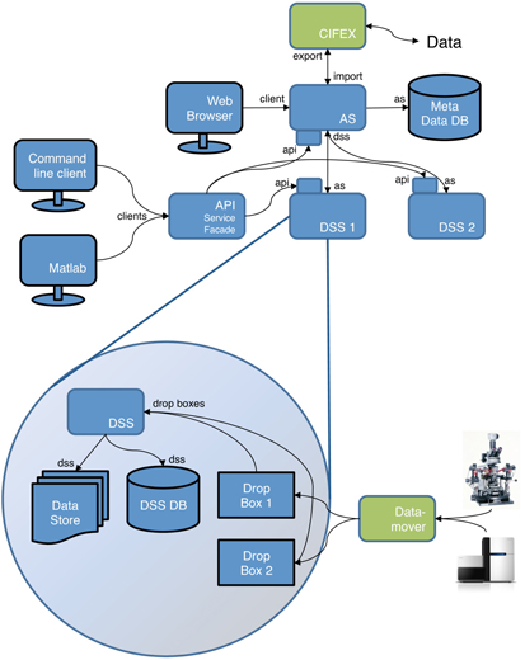
\includegraphics[width=0.7\textwidth]{openbis}
  \caption[Overview of the openBIS architecture and a more in-depth look at the data storage implementation.]{An openBIS instance is deployed as a service consisting of an application server (AS) and one or more data store servers (DSSs). At both levels, clients can interact with the system to query, fetch or deposit data. \citep{Bauch2011}.}
  \label{fig:openbis}
\end{figure}

\subsection{User Accessible Data Storage (OpenBIS)}


\section{Single Cell Feature Data}
\label{sec:scf-data}

\section{Infection Scoring}
\label{sec:infection-scoring}

\begin{figure}
\centering
\begin{tikzpicture}

\node [decision={$> 0.075$}{$\le 0.075$}] {
  \texttt{Cells.Intensity\_MeanIntensity\_\\CorrPathogen}
}
[decision tree]
child { node [outcome] { infected } }
child { node [decision={$> 0.085$}{$\le 0.085$}] { 
\texttt{PeriNuclei.Intensity\_MeanIntensity\_\\CorrPathogen} } 
  child { node [outcome] { infected } }
  child { node [decision={$> 0.115$}{$\le 0.115$}] { 
  \texttt{Nuclei.Intensity\_MeanIntensity\_\\CorrPathogen} } 
    child { node [outcome] { infected } }
    child { node [outcome] { not infected } }
  }
};

\end{tikzpicture}
\caption[Decision tree for adenovirus infection scoring.]{For adenovirus infection scoring, the decision tree classifier checks if enough pathogen is detected within the cell body, the perinuclear region or the nucleus. The threshold decreases as the region of interest concentrates on areas associated with progressively involved in infection.}
\end{figure}

\begin{figure}
\centering
\begin{tikzpicture}

\node [decision={$> 0.800$}{$\le 0.800$}] { 
  \texttt{Invasomes.Intensity\_MaxIntensity\_\\Corr1Pathogen}
}
[decision tree]
child { node [outcome] { infected } }
child { node [decision={$> 0.075$}{$\le 0.075$}] { 
\texttt{Invasomes.Intensity\_MeanIntensity\_\\Corr1Pathogen} } 
  child { node [outcome] { infected } }
  child { node [decision={$> 0.085$}{$\le 0.085$}] { 
  \texttt{Invasomes.Intensity\_UpperQuartile-\\Intensity\_Corr1Pathogen} }
    child { node [outcome] { infected } }
    child { node [decision={$> 12.00$}{$\le 12.00$}] { 
    \texttt{Invasomes.AreaShape\_Area} }
      child { node [decision={$< 1000$}{$\ge 1000$}] { 
        \texttt{Invasomes.AreaShape\_Area} }
        child { node [decision={$< 0.060$}{$\ge 0.060$}] { 
          \texttt{Invasomes.RadialDistribution\_FracAtD\_\\Corr1Actin\_1} }
          child { node [outcome] { infected } }
          child { node [outcome] { not infected } }
        }
        child { node [outcome] { not infected } }
      }
      child { node [outcome] { not infected } }
    }
  }
};

\end{tikzpicture}
\caption[Decision tree for \textit{Bartonella} infection scoring.]{Decision tree for \textit{Bartonella} infection scoring. In order to detect bona-fide invasomes, the first three or-linked decisions assemble a list of candidates while the following three and-linked decisions discard some erroneously included instances. In order to obtain the desired cell-based infection score, invasomes are mapped to cellular objects in a subsequent step.}
\end{figure}
